
\documentclass{article}

\usepackage{siunitx}
\usepackage{graphicx}
\usepackage{amsmath}
\usepackage{csquotes}
\usepackage[hidelinks]{hyperref}
\usepackage{xurl}
\usepackage{biblatex}
\usepackage{pgfplots}
\pgfplotsset{compat=1.18}

\setcounter{biburllcpenalty}{7000}
\setcounter{biburlucpenalty}{8000}

\addbibresource{references.bib}

\begin{document}
  \begin{titlepage}

    \begin{center}
      \includegraphics[width=8cm,height=3cm]{~/Documents/UIMP/comun/logo.jpg}
    \end{center}

    \vspace*{2cm}
    \begin{center}
      \Huge Resolución de problemas con metaheurísticos
    \end{center}

    \vspace*{2cm}
    \begin{center}
      \Large Trabajo final de la asignatura: trabajo 3.7 \\
      \large  Comparación de un algoritmo poblacional y uno de trayectoria \\
      \large Problema del $p$-hub
    \end{center}

    \vspace*{5cm}
    \noindent\rule{\textwidth}{0.4pt}
    \noindent Antonio González Cantizano \\
    Diciembre 2025

  \end{titlepage}

  \tableofcontents
  \newpage

  \section{Introduction}

  \hspace*{1em} The objective of this paper is to compare the Genetic Algorithm (GA) and Simulated Annealing (SA) 
  metaheuristics applied to the \textit{Uncapacitated Single Allocation p-Hub Median Problem (USApHMP)}. 
  The \textit{USApHMP} \cite{phub} is a combinatorial optimization problem where a set of nodes must be interconnected through a network of $p$ hubs. 
  Each node is allocated to exactly one hub, while hub nodes are allocated to themselves. 
  The primary goal is to minimize the following fitness function: 

  \begin{equation*}
    \text{Fitness} = \sum_{i \in N} \sum_{j \in N} w_{ij} \Big[ 
      c \cdot d_{ih_i} + t \cdot d_{h_i h_j} + d \cdot d_{h_j j} 
    \Big]
  \end{equation*}

  \noindent
    \text{where:}
    \begin{itemize}
      \item $N$ is the set of nodes.
      \item $H \subseteq N$ is the set of hubs.
      \item $h_i \in H$ is the hub assigned to node $i$.
      \item $w_{ij}$ is the flow between nodes $i$ and $j$.
      \item $d_{ij}$ is the distance between nodes $i$ and $j$.
      \item $c$, $t$, and $d$ are the collection, transfer, and distribution costs respectively.
    \end{itemize}

    For the different instances of the problem used in this study \cite{phub}, the flow matrix is allways asymmetric and features a non-null diagonal. 
    This implies that $w_{ij} \neq w_{ji}$ and $w_{ii} \neq 0$.\\ 
    \hspace*{1em} The implemented code and result sheets are provided alongside this paper.
  

  \section{Genetic Algorithm}
  \hspace*{1em} The GA was developed by adapting a generic implementation of the GA metaheuristic \cite{gitGA}. 
  For this work, the following configurations were selected based on \cite{sun}:
  \begin{description}
    \item \textbf{Solution Representation}: Each solution is represented as a tuple containing a list of hubs and a list of allocations. 
      The first list identifies the nodes selected as hubs, while the allocation list indicates which hub is assigned to each node.
    \item \textbf{Initial Population}: Each initial solution is generated through a two-step process: first, $p$ hubs are randomly selected; then, each node is allocated to its nearest hub. 
      This approach ensures a diverse set of initial solutions that cover a significant portion of the solution space while maintaining solution coherence, preventing the algorithm from wasting evaluations on low-quality candidates.
    \item \textbf{Parent Selection}: Selection is performed using a binary tournament approach.
    \item \textbf{Elitism}: An elitist strategy is employed to update the population across successive generations.
    \item \textbf{Crossover}: Hubs and allocations are combined using a single-point crossover strategy. 
      In cases where crossover disrupts the consistency of the solution (e.g., if a hub is removed from the hub list but remains in the allocation list), a repair mechanism is applied. 
      These unallocated nodes are re-allocated to their nearest available hub to maintain consistency.
    \item[Mutation]: First, two non-hub nodes are selected, and their allocations are swapped. 
      Next, another non-hub node is selected and its allocation is changed to a random hub. 
      Refer to Figure \ref{fig:crossover} for a visual example.
  \end{description}

  \begin{figure}
    \centering
    \includegraphics[width=12cm,height=5cm]{./images/crossMutt.png}\\
    \caption{An example of crossover and mutation \cite{sun}}
    \label{fig:crossover}
  \end{figure} 

  \subsection{Parameter Selection}
  \hspace*{1em} Following implementation, a refinement process was conducted to optimize the GA parameters. 
  A total of 400 executions were performed, varying the population size and mutation probability across problems of different sizes. 
  The average fitness and the frequency with which a specific combination reached the minimum value within the test set have been 
  used in order to select the best tuple of parameters. With the maximum number of evaluations fixed at 10000, values of 200 for population size and 0.05 for mutation probability were chosen (see Table \ref{table:table1}).

    \begin{table}
      \centering
      \begin{tabular}{ c S c r}
        {Population size} & {Mutation prob} & {Average fitness} & {Best} \\
        \hline
        10 & 0.01 & 161758783 & 0\\  
        10 & 0.05 & 163395834 & 2\\  
        10 & 0.1 & 164796836 & 2\\  
        10 & 0.2 & 164624940 & 2\\  
       50 & 0.01 & 150852033 & 5\\  
       50 & 0.05 & 150401498 & 5\\  
       50 & 0.1 & 150537436 & 5\\  
      50 & 0.2 & 150537436 & 4\\  
      100 & 0.01 & 148652430 & 5\\  
      100 & 0.05 & 147763095 & 7\\  
      100 & 0.1 & 147997723 & 8\\  
      100 & 0.2 & 147913642 & 10\\  
      150 & 0.01 & 146795895 & 8\\  
      150 & 0.05 & 146922234 & 9\\  
      150 & 0.1 & 147060801 & 9\\  
      150 & 0.2 & 146563806 & 11\\  
      200 & 0.01 & 146925144 & 7\\  
      200 & 0.05 & 146169925 & 11\\  
      200 & 0.1 & 146494179 & 10\\  
      200 & 0.2 & 146662319 & 9\\  
      \end{tabular}
      \caption{Results of the parameter selection for the GA algorithm}
      \label{table:table1}
    \end{table}

  \section{Simulated Annealing}
  \hspace*{1em} The Simulated Annealing implementation follows the approach described by \cite{ernst}, with a primary focus on neighbor selection. 
  Three mechanisms for generating neighbors were implemented:
  \begin{description}
    \item \textbf{Swap}: With a probability of 0.4, this operator is chosen to generate a neighbor by re-assigning a random non-hub node to a different random hub.
    \item \textbf{Move}: With a probability of 0.6, a hub (cluster) is selected for modification:
      \begin{description}
        \item \textbf{If the cluster is a singleton}: A random non-hub node is chosen to become the new hub of this cluster, and the previous hub is allocated to it. 
          As singleton clusters are rarely part of optimal solutions, this operator ensures the algorithm escapes these sub-optimal configurations.
        \item \textbf{Otherwise}: A random node within the selected cluster is chosen to become the new hub. The previous hub and all nodes of the cluster are then re-allocated to this new hub.
      \end{description}
  \end{description}
  

  \subsection{Parameter selection}
  \hspace*{1em} According to the methodology in Section 2.1, the number of iterations was fixed at 10000 and the same instances were used. 
  The number of iterations per temperature level ($l$) is determined as:
  \begin{equation*}
    l = \frac{10000}{\text{Initial temperature}} 
  \end{equation*}
  \hspace*{1em} This ensures exactly 10000 fitness evaluations. For the final model, an initial temperature of 1000 and a cooling coefficient of 0.9 were selected based on the results of the Table \ref{table:table2}

  \begin{table}
    \centering
    \begin{tabular}{ c S c r}
      {Initial temp} & {Cooling coef} & {Average fitness} & {Best}\\ 
      \hline
      100 & 0.85 & 149238092 & 10\\  
      100 & 0.9 & 150721776 & 3\\  
      100 & 0.95 & 149547568 & 7\\  
      100 & 0.97 & 149639708 & 8\\  
      1000 & 0.85 & 149291239 & 9\\  
      1000 & 0.9 & 148526968 & 10\\  
      1000 & 0.95 & 152848812 & 4\\  
      1000 & 0.97 & 150440420 & 7\\  
    \end{tabular}
      \caption{Results of the parameter selection for the SA algorithm}
      \label{table:table2}
  \end{table}

  \section{Comparison}
  \hspace*{1em} To compare both algorithms, parameters were fixed and 23 problem instances were tested. 
  Both models were limited to 10,000 fitness evaluations to ensure a fair comparison. 
  For each instance, the results represent the average fitness over 4 independent runs. 
  Execution times were also recorded. Representative results are shown in Table \ref{table:table3} (full data available in the shared .ods file).

  \begin{table}
    \centering
    \begin{tabular}{ c c c c c}
      {Algorithm} & {N} & {P} & {Average fitness} & {Time (ms)}\\
      \hline
      GA & 10 & 2 & 167493064 & 124 \\  
      SA & 10 & 2 & 168504989 & 6.25 \\ 
      GA & 20 & 5 & 123366722 & 75.5 \\ 
      SA & 20 & 5 & 126174633 &  21.75 \\ 
      GA & 200 & 9 & 122838852 &  2217 \\ 
      SA & 200 & 9 & 124709811 &  2166.5 \\ 
    \end{tabular}
      \caption{Some example of the comparison between the GA and the SA}
      \label{table:table3}
  \end{table}

  \subsection{Fitness comparison: Wilcoxon signed-rank test}

  \hspace*{1em} Given that the results comprise 23 pairs of results and non-parametric fitness values, the Wilcoxon signed-rank test was employed to determine if one model significantly outperforms the other, following guide \cite{wilcoxon}. 
  The difference is defined as:
  \begin{equation*}
    \Delta_{Fi} = F_{Gi} - F_{Si}
  \end{equation*}

  Where $F_{Mi}$ is the average fitness for model $M$ and instance $i$. 
  A bilateral test was conducted with the following hypotheses:

  \[
    \begin{aligned}
      H_0 &: \operatorname{median}(\Delta_{Fi}) = 0, \\
      H_1 &: \operatorname{median}(\Delta_{Fi}) \neq 0.
    \end{aligned}
  \]

  Ranks were assigned based on the absolute values of the differences. The table \ref{table:table4} summarizes the ranking (note: instances where $\Delta_{Fi} = 0$ are excluded, resulting in $n=22$):


  \begin{table}
    \centering
    \begin{tabular}{ c c c}
      Sign & $\Delta_{Fi}$ & Rank \\
      \hline
      - & 105552 & 1 \\ 
      - & 190121 & 2 \\ 
      - & 1011924 & 3 \\ 
      - & 1162282 & 4 \\ 
      - & 1279529	& 5 \\ 
      - & 1410758	& 6 \\ 
      - & 1451492	& 7 \\ 
      - & 1648498	& 8 \\ 
      - & 1870959	& 9 \\ 
      - & 2197516	& 10 \\ 
      - & 2241400	& 11 \\ 
      - & 2807910 & 12 \\ 
      - & 2857826 & 13 \\ 
      - & 2972416	& 14 \\ 
      + & 3068732	& 15 \\ 
      - & 3313670	& 16 \\ 
      - & 4470062	& 17 \\ 
      - & 4667384	& 18 \\ 
      - & 7461131	& 19 \\ 
      - & 9003728	& 20 \\ 
      - & 9740489	& 21 \\ 
      - & 13402391 & 22 \\
    \end{tabular}
    \caption{Wilcoxon ranking for $\Delta_{Fi}$}
    \label{table:table4}
  
  \end{table}
  
   Ranks are added to obtain $W_- = 238$ and $W_+ = 15$, with $\min(W_-, W_+)$ = 15. 
   Looking at the Wilcoxon signed-rank test critical values table \cite{wilTable}, for $n=22$ and $\alpha = 0.01$ the critical value for a bilateral test is 48. 
   Since $15 < 48$, we reject $H_0$ with 99\% significance. 
   Given $W_- > W_+$, we confirm $F_{G} < F_{S}$, indicating that the GA consistently achieves lower average fitness than SA for the tested instances.

  \subsection{Time comparison}
  \hspace*{1em} Applying the same statistical approach to execution time differences, $\Delta_Ti$ is defined as:
  \begin{equation*}
    \Delta_{Ti} = T_{Gi} - T_{Si}
  \end{equation*}

\begin{figure}[h]
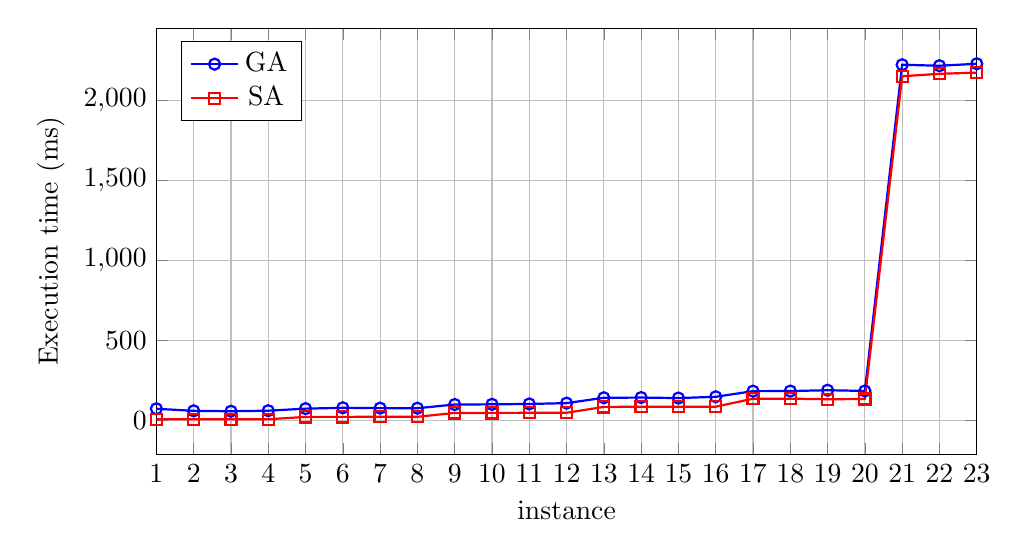
\begin{tikzpicture}
\begin{axis}[
    width=12cm,
    height=7cm,
    xlabel={instance},
    ylabel={Execution time (ms)},
    xtick={1,2,...,23},
    xmin=1, xmax=23,
    grid=both,
    legend pos=north west,
]

% Modelo 1
\addplot[
    color=blue,
    mark=o,
    thick
]
coordinates {
    (1,72) (2, 59) (3, 56.5) (4, 60) (5, 72.75)
    (6, 78) (7, 76) (8,75.5) (9,98.5) (10,99.75)
    (11,102) (12,107.25) (13,140.75) (14,142) (15,139)
    (16,146.75) (17,182.25) (18,182.75) (19,188) (20,183.5)
    (21,2223) (22,2217) (23,2229.25)
};
\addlegendentry{GA}

% Modelo 2
\addplot[
    color=red,
    mark=square,
    thick
]
coordinates {
    (1,6.25) (2,6) (3,6.25) (4,6.25) (5,21.25)
    (6,21.25) (7,21.75) (8,21.75) (9,46) (10,46.25)
    (11,46.5) (12,46.75) (13,83.75) (14,84.25) (15,84.75)
    (16,85) (17,135) (18,135.25) (19,131.5) (20,133)
    (21,2151.25) (22,2166.5) (23,2174)
};
\addlegendentry{SA}

\end{axis}
\end{tikzpicture}
\caption{Comparison of the execution time for the GA and SA}
\label{fig:2}

\end{figure}

  We observed in figure \ref{fig:2} that $\Delta_{Ti}$ is allways positive ($W_- = 0$). 
  This allows us to affirm without proceeding with the Wilcoxon test that SA is significantly faster than GA for these instances.
  The execution time difference between the GA and the SA remains approximately constant at around 50 ms ($47 < \Delta_{Ti} < 72$ ms) and does not increase with the problem size, suggesting a fixed cost inherent to the GA, such as the initialization and evaluation of the initial population.

  \section{Conclusions}

  \hspace*{1em} This study demonstrates that the Genetic Algorithm consistently finds superior solutions compared to Simulated Annealing for the \textit{USApHMP}. 
  This is likely due to the GA's ability to maintain a population (200 individuals) that explores a larger segment of the solution space. 
  While SA behaves more like a local search with the ability to escape local minima, its search trajectory becomes increasingly constrained as the temperature decreases. 
  In contrast, GA maintains diversity through crossover and mutation. 
  Even in small instances, GA reached the global minimum more reliably.
  
  The time difference, while statistically significant, is not proportional to problem size and likely represents a fixed setup cost for the GA. 
  In terms of resources, SA remains a viable alternative for memory-constrained environments, such as embedded systems, as it only tracks a single solution. 
  However, for all other cases where memory permits, the use of a Genetic Algorithm is recommended for this problem class.

  \newpage
  \printbibliography

\end{document}
